\documentclass{article}
\usepackage[utf8]{inputenc}
\usepackage{diffcoeff}  
\usepackage{amsmath}
\usepackage{amssymb}
\usepackage{cancel}
\usepackage{nicefrac}
\usepackage{graphicx}
\usepackage{geometry}
\usepackage{authblk}
\geometry{letterpaper, top=25mm, bottom=25mm, left=25mm, right=25mm}


\title{Modelling The Flow of Crowds}
\author{Katya Driscoll, \"Ozge G\"ulsay{\i}n, Ciaran Neely, Wardah Ur-Rehman}

\begin{document}
\maketitle

\section{Introduction}
Two fundamental frameworks have been proposed to model crowd motion. The first treats pedestrians as discrete individuals, allowing for each person's behaviour to be defined separately. This gives the model a great deal of flexibility. Generally, computers are used to precisely simulate the crowd under a specific set of circumstances. This model is best suited to small, less dense clusters of people, and lacks the ability to provide us with general results on crowd behaviour. Conversely, the second framework, analyzed in this paper, observes the crowd as a whole and treats it like a continuum. Unlike in the first model, the individuals involved all follow the same general behavioural pattern: moving as efficiently as possible to reach their objectives. This makes it better suited to larger, denser crowds, whose behaviour approximate a continuum.

\section{Derivation}
\subsection{Physical Assumptions}
\newcommand\Rpix{\mathcal R_{\text{\texttt{px}}}}
\newcommand{\brydon}{\texttt{Brydon}}
In order to go about modelling something as complex as a group of human individuals, we must make a few simplifying assumptions. Let $\mathcal R\subseteq\mathbb R^2$ be an arbitrary region in space with a smooth boundary, where the crowd operates. Firstly, we must assume that the crowd is dense enough that its behaviour mimics a continuum, or our model will be inaccurate. In other words, there are enough people per unit area such that $\mathcal R$ is a nonempty, compact, and connected space. We also assume there are no inanimate obstacles in the crowd large enough to significantly affect the overall flow of people. Finally, we restrict the crowd to operating in only 2 spatial dimensions. Physically, this means that the ground on which the crowd operates is approximately flat, and that people remain close enough to the ground. Hence, our overall model will have 3 independent variables: $x$, $y$ (spatial), and $t$ (temporal).

\subsection{Conservation of Pedestrians}
We start by assuming that in a given area of the crowd, the flow of the pedestrians is conserved. Then, we can set up the skeleton of our PDE by using the conservation law. 

\begin{enumerate}
    \item Based on the assumption of the crowd acting as a continuum, we can define $\rho$, the density of the "flow" of pedestrians per unit area, at a given time $t$.
    \item This flow of pedestrians would also have a  velocity $\vec{v}$ (in directions $x$, $y$) at a given time, at a given location.
    \item For our purposes, we will also assume that there is no creation nor destruction of pedestrians.
\end{enumerate}

Therefore, using our local conservation law, we get the following PDE:

\begin{equation}
    \diffp \rho t = - \nabla\cdot (\rho\vec v)
\end{equation}



\subsection{Modelling Behaviour}
In this section, we define the basic behaviour of pedestrians to give their movement a necessary degree of predictability. The following 3 hypotheses frame this behaviour:
\begin{enumerate}
    \item \textbf{Hypothesis 1:} The speed at which any individual pedestrian will walk depends only on the density of their surroundings. In other words, under a particular set of circumstances, any individual from the crowd will move at the same speed, regardless of personality or height.
    \\
    This hypothesis defines that for our conservation law, we can have that velocity function is only a function of $\rho$.
    \begin{equation}
        \vec{v} = v(\rho) \hat{v}\label{hyp1}
    \end{equation}
    
    
    \item \textbf{Hypothesis 2:} Each individual has a `goal' (referred to as `potential'), or a place they want to get to. We can model this by assigning a `potential' $\phi(\vec x)$ to each location $\vec x \in\mathcal R$. We assume that each person moves to minimize their potential as efficiently as possible. This leads to the following equation,  which tells us how individuals choose their direction of movement.
    \\
    Mathematically speaking, minimizing the potential means moving perpendicular to the ``potential", which determines our direction vector as the normal vector to the potential function:
    \begin{equation}
         \hat{v} = \hat{n} = -\frac{\nabla\phi(\vec x)}{\|\nabla\phi(\vec x)\|}
    \end{equation}
    
    \item \textbf{Hypothesis 3:} Pedestrians seek to minimize their travel time, while avoiding highly dense clusters of people. The Triangle Inequality tells us that the quickest way to get from point A to point B is to travel in a straight line. In this scenario, individuals abide by this principle, while also taking small detours to avoid highly dense areas in the crowd. To describe this individual path, we will introduce a proportionality function $g(\rho)$, which accounts for these detours.
    
    So we have that distance between the two potentials are proportional to the speed of the flow of pedestrians and $g(\rho)$ , which we can interpret as some factor to allow for discomfort at high densities:
    \begin{equation}
        g(\rho) f(\rho) = \frac{1}{ \sqrt{ \left(\frac{\partial \phi}{\partial x} \right)^2 + \left(\frac{\partial \phi}{\partial y} \right)^2 } }
    \end{equation}
    
    
    
    The equations from the 3 hypotheses come together to form the final version of our PDE for pedestrian flow.
    \begin{equation}
        -\frac{\partial \rho}{\partial t} + \frac{\partial}{\partial x} \left(\rho g(\rho) f^2 (\rho) \frac{\partial \phi}{\partial x} \right) + \frac{\partial}{\partial y} \left(\rho g(\rho) f^2 (\rho) \frac{\partial \phi}{\partial y} \right) = 0
    \end{equation}

    
    
    
    
\end{enumerate}

\section{Stability of the Front}
The PDE derived in the previous section has the potential to model many situations in the real world. From the annual Muslim Hajj to marathons that take place around the world. An interesting historical application is modelling the Battle of Agincourt.

\subsection{The Battle of Agincourt}
The Battle of Agincourt took place in France on October 25th, 1415 between the English and French armies. While details of the battle vary, modern accounts suggest the English had around 6000 to 7000 soldiers. Many soldiers were also weakened by illness and hunger due to previous battles. Comparatively, the French army had 2 lines of 8000 soldiers in each one. Along with around 9000 other soldiers. The battle ended with the English army's victory and a slain French ``wall of bodies" by modern accounts. Given the immensely greater and stronger French side, one would assume it would be the French's victory.

\subsection{Modelling the Battle}
Thus, to explore the events that took place at the front lines, researchers Clements \& Hughes (2004) modelled the front line using the equations derived for the flow of crowds. To set up the physical situation, the soldiers can be modelled as two separate human crowds, exhibiting different behaviours. As shown in Figure 1, the battle occurred between two woods around one kilometre apart; that is, in a confined space. \\
\begin{figure}[h]
\centering
\caption{Battle of Agincourt}
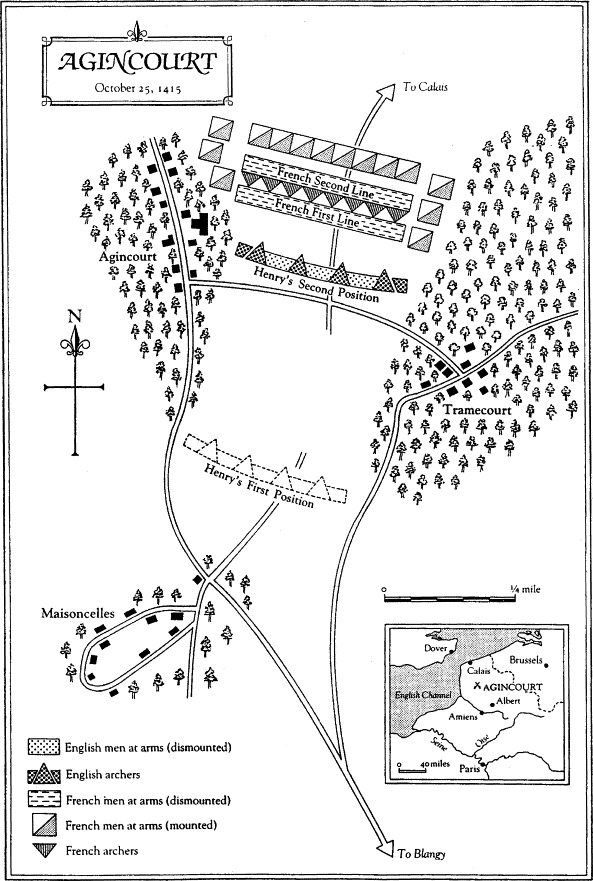
\includegraphics[width=0.4\textwidth]{battlefield.jpg}
\end{figure}
Further, given their numbers, the highly dense area fits with the physical assumptions and hypotheses of the continuum model discussed previously. Furthermore, Clements and Hughes denoted $\eta(x,t)$ as the line between the French forces coming from the North, denoted $y=L_f$, and the English from the south, denoted $y=-L_e$, as seen in Figure 2. \\
\begin{figure}[h]
\centering
\caption{Battle of Agincourt}
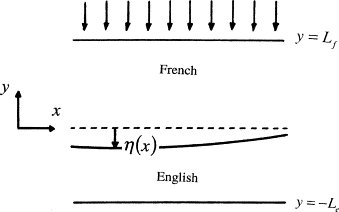
\includegraphics[width=0.4\textwidth]{mathmodel.jpg}
\end{figure}
\\
They then used the PDE to model the front line $\eta(x,t)$ and analyzed its stability using a technique known as ``perturbation series". 

\subsection{Perturbation Series and Stability}
Perturbation series is a way to approximate solutions as series of powers of $\varepsilon$. Though the full extent of how perturbation series were used to find the stability of $\eta$ is beyond the scope of this course, we can demonstrate a simpler example of how it was used. Consider the problem of finding $\sqrt{4.01}$. An equivalent problem is finding $a_0,a_1,...\in\mathbb R$ such that
\[
    (a_0+a_1\varepsilon+a_2\varepsilon^2+\cdots)^2=4+\varepsilon
\]
where $\varepsilon=0.01$. To find an approximate solution, we simply round $\varepsilon$ down to zero, then the problem becomes $a_0^2=4$, which we know the positive solution to be $a_0=2$. In order to improve our approximation, we will need to relax the assumption that $\varepsilon=0$. If we do this, we get
\begin{align*}
    &(2+a_1\varepsilon)^2=4+\varepsilon\\
    \implies& 4+4a_1\varepsilon+\cancel{a_1^2\varepsilon^2}=4+\varepsilon\\
    \implies& 4a_1\varepsilon=\varepsilon\\
    \implies& (4a_1-1)\varepsilon =0\\
    \implies& a_1=\nicefrac{1}{4}
\end{align*}
This gives us a first order approximation of the solution
\[
    \sqrt{4+0.01}\approx 2+\frac 14(0.01)=2.0025
\]
For reference, plugging the problem into a calculator produces $\sqrt{4.01}\approx 2.00249843945$, so $2.0025$ is already a pretty reasonable approximation. We can continue like this indefinitely getting a closer approximation each time. A useful byproduct of using this technique is that we actually have a general solution to the value of $\sqrt{4+\varepsilon}$ for $\varepsilon\le 1$. Namely
\[
    \sqrt{4+\varepsilon}=2+\tfrac 14\varepsilon-\tfrac 1{32}\varepsilon^2+O(\varepsilon^3)
\]
which tells us $\sqrt{4+\varepsilon}$ is greater than $\sqrt{4}$ (unless something bizarre happens for $a_3,a_4,...$). This makes perturbation series a valuable tool for stability analysis. For instance
\[
    y'=\sqrt y-2
\]
which has one steady-state at $y=4$. Is that steady state stable? Our second order approximation of $\sqrt{4+\varepsilon}$ suggests that it is not. Even if we start with $y=4$, in any real-world example, we should expect to see $y$ veer off wildly in one direction or the other, as even the smallest disturbance will cause it to do so.

\subsection{The Results}
By expressing $\rho$, $\vec v$, $\phi(\vec x)$, and $\eta$ as a series of coefficients on powers of $\varepsilon$, we can use a similar logic to find whether $\eta$ will remain stable over time. \\
\\
As Clements and Hughes found, the front line, $\eta(x,t)$, was in fact unstable. The instability caused openings to be formed in the front line, at $\eta=0$ in Figure 2. One side could then enter the other through these openings. The French being confident could charge through the openings, be surrounded by the English soldiers and be killed there. \\
\\
An interesting finding is that in modern accounts of the battlefield at the end is described as a ``wall of bodies" at the front line. However, this is inconsistent with the model. So historians researched further into this and discovered that in current times the battle was simply being described wrong. An in historical accounts, there isn't a ``wall" of bodies described. These findings show how powerful PDE models can be in various fields; such as history, which is often considered void of mathematics.

\section{References}
Bender, C. M., \& Orszag, S. A. (1978). \emph{Advanced mathematical methods for scientists and Engineers}. McGraw-Hill. 
\\\\
Clements, R. R., \& Hughes, R. L. (2004). \emph{Mathematical modelling of a mediaeval battle: The battle of Agincourt, 1415}. Mathematics and Computers in Simulation, 64(2), 259–269. https://doi.org/10.1016/j.matcom.2003.09.019 \\
\\
Hughes, R. L. (2002). \emph{A continuum theory for the flow of pedestrians}. Transportation Research Part B: Methodological, 36(6), 507–535. https://doi.org/10.1016/S0191-2615(01)00015-7 
\end{document}

